\chapter{Introduction}

Sparse Distributed Memory (SDM) \citep{Kanerva1988} is a mathematical model of long-term memory that has a number of neuroscientific and psychologically plausible dynamics. It has been applied in many different fields, like pattern recognition \citep{norman2003modeling, rao1995natural}, noise reduction \citep{Meng2009}, handwriting recognition \citep{fan1997genetic}, robot automation \citep{Rajesh1998, mendes2008robot}, and so forth. Despite all those applications, there is not a reference implementation which would allow one to replicate the results published in a paper, to check the source code for details, and to improve it. Thus, even though great results have been achieved using SDM, it requires great effort of researchers to improve someone's work.

It is our belief that this tool could bring orders of magnitude more researchers and attention if they were able to use the model, at zero cost, with an easy to use high-level language such as python. Neuroscientists interested in long-term memory storage should not have to worry about high-bandwidth vector parallel computation.  This new tool provides a ready to use system in which experiments can be executed almost as soon as they are designed.

Our motivation was our own effort in order to run our models. As there is no reference implementation, we had to implement our own and run several simulations to ensure that our implementation was correct and bug free. Thus, we had to deviate from our main goal --- which was to test our models --- and to focus in the implementation itself. Furthermore, new members in our research group had to go through different source codes developed by former members.

The main contribution of this work is a reference implementation which yields (i) orders of magnitude gains in performance, (ii) has several backends and operations, (iii) has automatic tests, (iv) is cross-platform, and (v) is easily extended to fulfill other research models. Our reference implementation may, hopefully, accelerate research into the model's dynamics and make it easier to readers to replicate any previous results and easily understand the source-code of the model.


\chapter{Sparse Distributed Memory}

% !TEX root = ../partial-sdm.tex

Sparse Distributed Memory (SDM) is a mathematical model for cognitive memory published by \citet{Kanerva1988}. It introduces many interesting mathematical properties of $n$-dimensional binary space that, in a memory model, are psychologically plausible.  Most notable among these are the tip-of-the-tongue phenomenon, conformity to Miller's magic number \citep{Linhares2011} and robustness against loss of neurons.

The data and address space belong to binary space and are represented by a sequence of bits, called bitstrings. The distance between two bitstrings is calculated using the Hamming distance. It is defined for two bitstrings of equal length as the number of positions at which the bits are different. For example, $00110_{b}$ and $01100_{b}$ are bitstrings of length 5 and their Hamming distance is 2. One has to be careful when thinking intuitively about distance in SDM because the Hamming distance does not have the same properties of, say, the Euclidean distance.

\begin{figure}[p!]
  \centering
  \subfloat[$Q_3$]{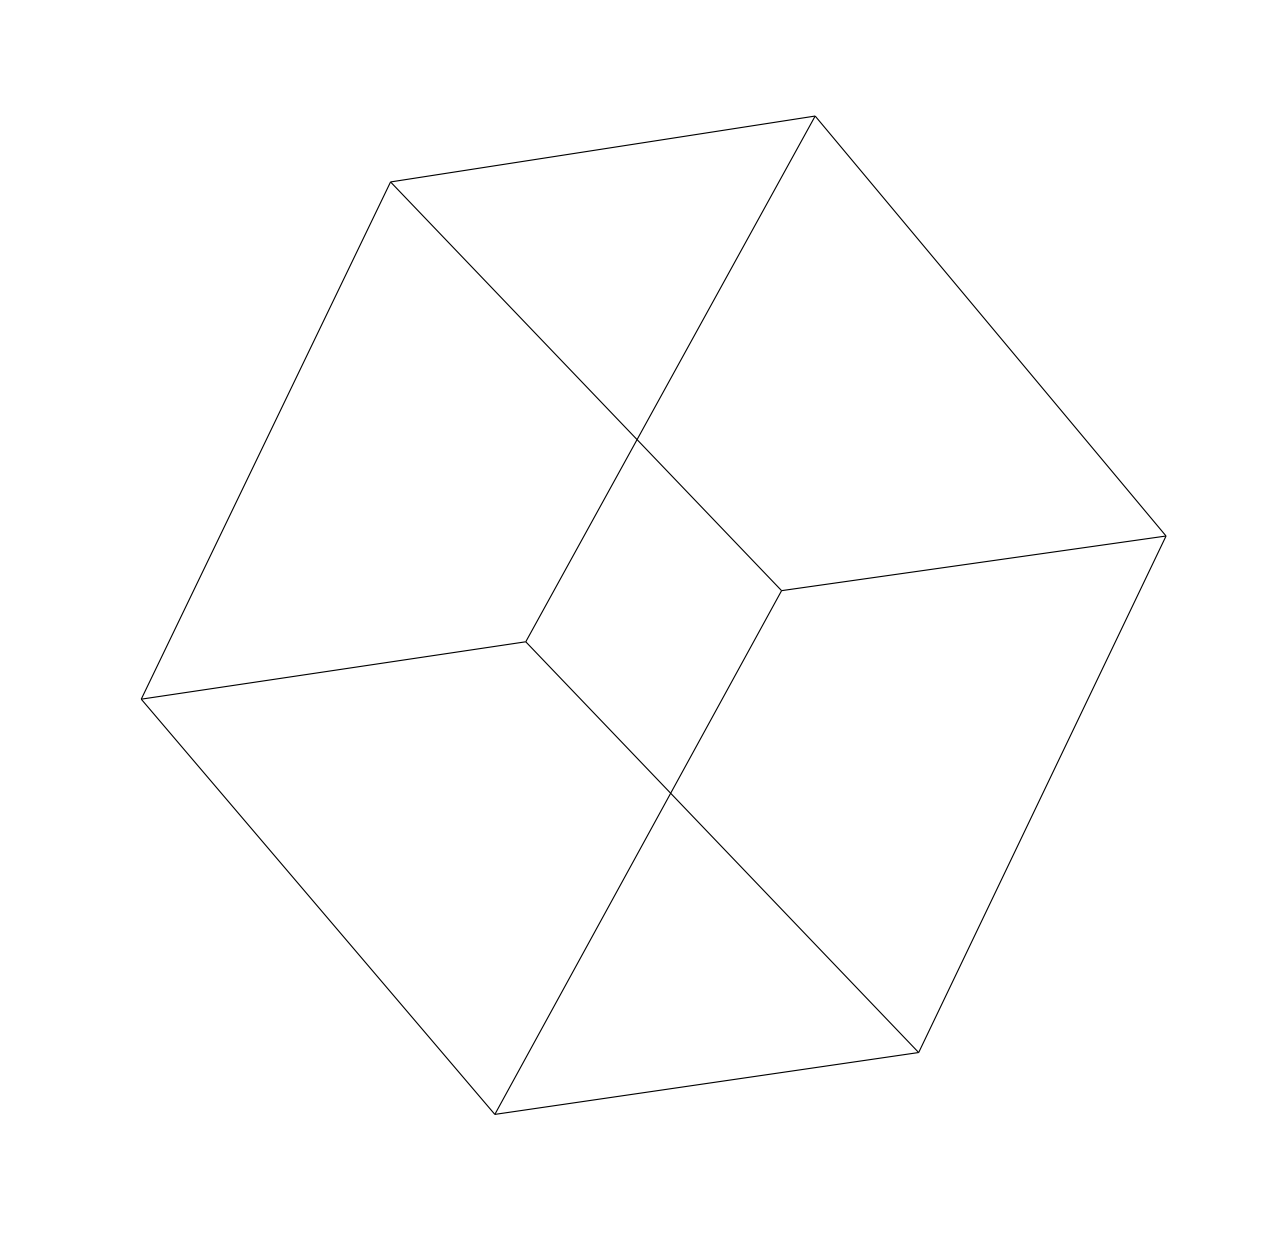
\includegraphics[width=2.2in]{./images02/new-images/qn3.png}}
  \subfloat[$Q_7$]{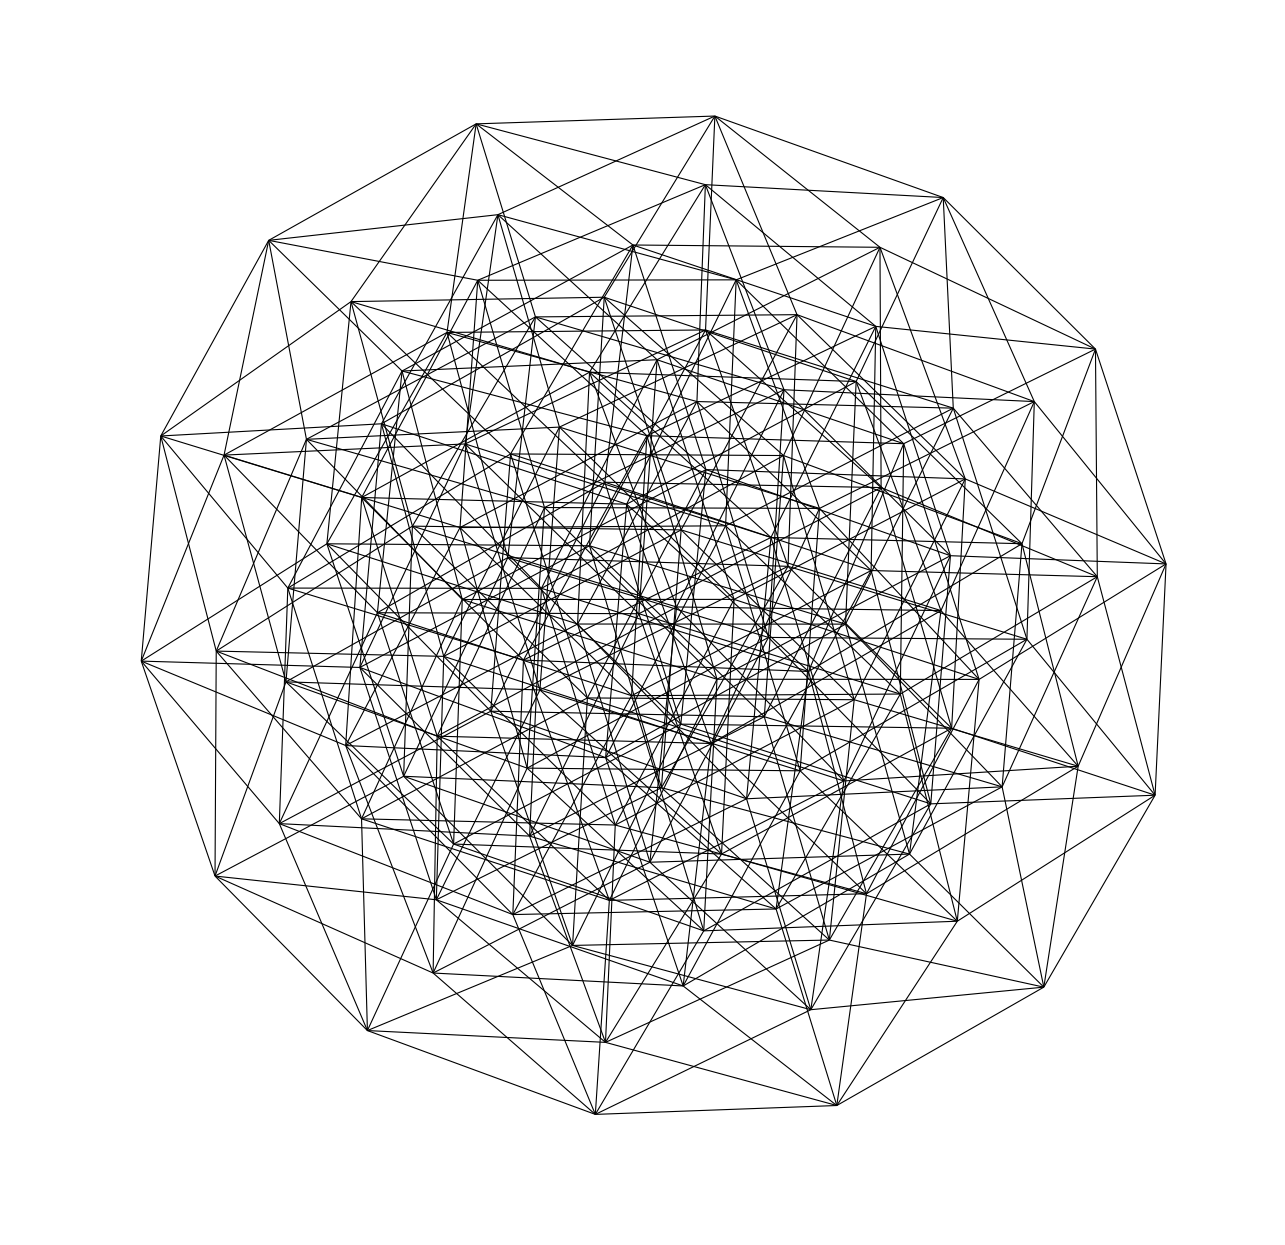
\includegraphics[width=2.2in]{./images02/new-images/qn7.png}}

  \subfloat[$Q_{10}$]{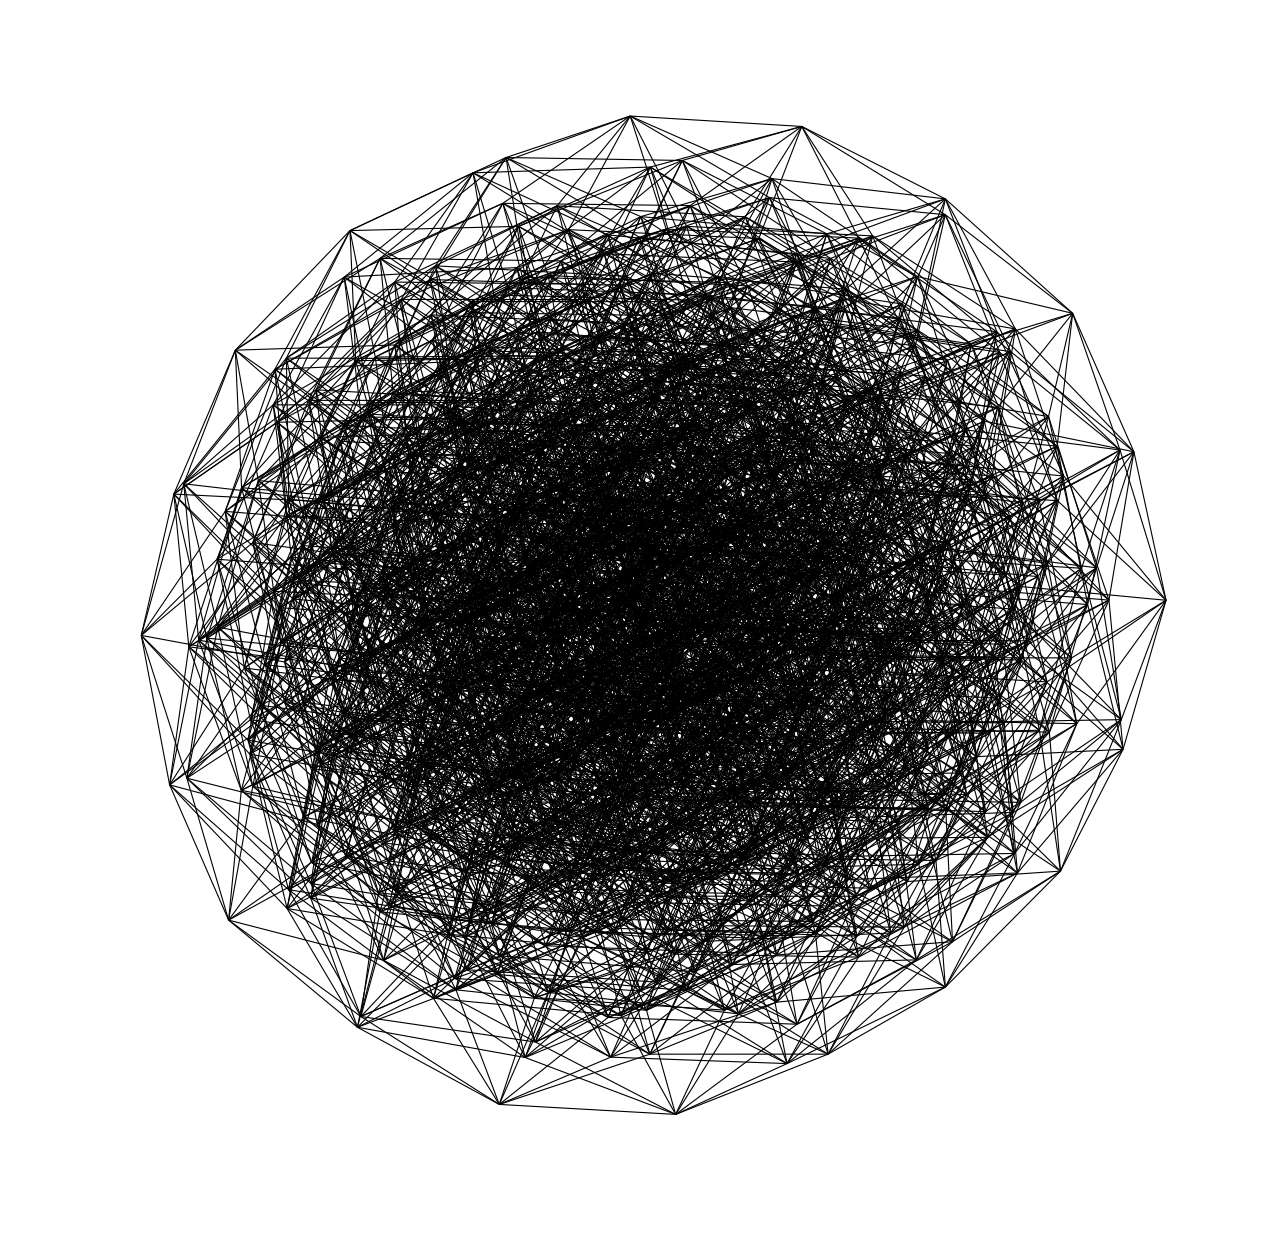
\includegraphics[width=4.0in]{./images02/new-images/qn10.png}}
  \caption{Here we have $Q_n$, for $n \in$ \{3, 7, 10\}. Each node represents a possible bitstring in $\{0,1\}^n$, and two nodes are linked if the bitstrings differ by a single dimension.  A number of observations can be made here. First, the number of nodes grows as $2^n$ as $n$ grows; which makes use of the entire space infeasible as $n>>20$. Another interesting observation, better seen in the figures below, is that most of the space lies at the center, at a distance of around 500 from any given vantage point.\label{hypercubes}}
\end{figure}



The graph composed of $\{0,1\}^n$ nodes and links between nodes $iff$ their Hamming distance is one is called the \emph{hypercube graph}, or $Q_n$, as in Figure \ref{hypercubes}.  Though Kanerva has derived many combinatorial properties of the space, I believe that this is a aesthetically appealing object on its own, and beautiful results can be found in the graph-theoretical literature. A good survey is found in \citet{harary1988survey}.


Here is an interesting question that I leave for further research: A hypercube with n dimensions can be divided by two hypercubes with $n-1$ dimensions. Is there an algorithm that separates the area of each hard-location in such a form that there exists a function mapping each bitstring in $\{0,1\}^n$ to the set of hard locations it belongs to?  In other words… though this would break Kanerva's assumption of a uniformly distributed set of hard locations for a perfectly symmetrical set of hard locations, there could be large performance gains if such a mapping function from a bitstring to its corresponding set of nearest hard locations exists.





Unlike traditional memory used by computers, SDM performs read and write operations in a multitude of addresses, also called neurons.  That is, the data is not written, or it is not read in a single address spot, but in many addresses. These are called activated addresses, or activated neurons.

The activation of addresses takes place according to their distances from the datum. Suppose one is writing datum $\eta$ at address $\xi$, then all addresses inside a circle with center $\xi$ and radius $r$ are activated. So, $\eta$ will be stored in all these activated addresses, which are around address $\xi$, such as in Figure \ref{fig-addresses-inside-access-radius}.  An address $\xi'$ is inside the circle if its hamming distance to the center $\xi$ is less than or equal to the radius $r$, i.e. $distance(\xi,\xi')\leq r$.

\begin{figure}[!htb]
\centering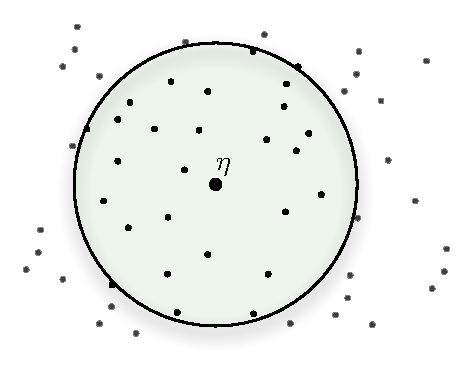
\includegraphics[scale=0.75]{./images02/p_circle_r.pdf}

\caption{Activated addresses inside access \protect \\
radius $r$ around center address.\label{fig-addresses-inside-access-radius}}
\end{figure}



Every time write or read in SDM memory activates a number of addresses with close distance.  The data is written in these activated addresses or read from them.  These issues will be addressed in due detail further on, but a major difference from a traditional computer memory is that the data are always stored and retrieved in a multitude of addresses. This way SDM memory has robustness against loss of addresses (e.g., death of a neuron).

In traditional memory, each datum is stored in an address and every look up of a specific datum requires a search through the memory. In spite of computer scientists having developed beautiful algorithms to perform fast searches, almost all of them do a precise search. That is, if you have an imprecise clue of what you need, these algorithms will simply fail.

In SDM, the data space is the same as the address space, which amounts to a vectorial, binary space, that is, a $\{0,1\}^{n}$ space. This way, the addresses where the data will be written are the same as the data themselves. For example, the datum $\eta=00101_{b}\in\{0,1\}^{5}$ will be written to the address $\xi=\eta=00101_{b}$. If one chooses a radius of 1, the SDM will activate all addresses one bit away or less from the center address. So, the datum $00101_{b}$ will be written to the addresses $00101_{b}$, $10101_{b}$, $01101_{b}$, $00001_{b}$, $00111_{b}$, and $00100_{b}$.

In this case, when one needs to retrieve the data, one could have an imprecise cue at most one bit away from $\eta$, since all addresses one bit away have $\eta$ stored in themselves.  Extending this train of thought for larger dimensions and radius, exponential numbers of addresses are activated and one can see why SDM is a distributed memory.

When reading a cue $\eta_{x}$ that is $x$ bits away of $\eta$, the cue shares many addresses with $\eta$. The number of shared addresses decreases as the cue's distance to $\eta$ increases, in other words, as $x$ increases. This is shown in Figure \ref{fig-shared-addresses}.  The target datum $\eta$ was written in all shared addresses, thus they will bias the read output in the direction of $\eta$. If the cue is sufficiently near the target datum $\eta$, the read output will be closer to $\eta$ than $\eta_{x}$ was. Repeating the read operation increasingly gets results closer to $\eta$, until it is exactly the same. So, it may be necessary to perform more than one read operation in order to converge to the target data $\eta$.

\begin{figure}[!htb]
\centering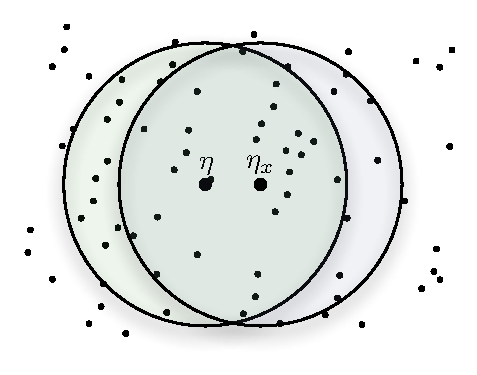
\includegraphics[scale=0.75]{./images02/p1_inter_p2.pdf}

\caption{Shared addresses between the \protect \\
target datum $\eta$ and the cue $\eta_{x}$. \label{fig-shared-addresses}}
\end{figure}


The addresses of the $\{0,1\}^{n}$ space grows exponentially with the number of dimensions $n$, i.e. $N=2^{n}$. For $n=100$ we have $N\approx10^{30}$, which is incredibly large when related to a computer memory. Furthermore, \citet{Kanerva1988} suggests $n$ between 100 and 10,000. Recently he has postulated 10,000 as a desirable minimum $N$ (personal communication). To solve the feasibility problem of implementing this memory, Kanerva made a random sample of $\{0,1\}^{n}$, in his work, having $N'$ elements. All these addresses in the sample are called hard-locations. Other elements of $\{0,1\}^{n}$, not in $N'$, are called virtual neurons. This is represented in Figure \ref{fig-hardlocations}.  All properties of read and write operations presented before remain valid, but limited to hard-locations. Kanerva suggests taking a sample of about one million hard-locations.

Using this sample of binary space, our data space does not exist completely.  That is, the binary space has $2^{n}$ addresses, but the memory is far away from having these addresses available. In fact, only a fraction of this vectorial space is actually instantiated. Following Kanerva's suggestion of one million hard-locations, for $n=100$, only $100\cdot10^{6}/2^{100}=7\cdot10^{-23}$ percent of the whole space exists, and for $n=1,000$ only $100\cdot10^{6}/2^{1000}=7\cdot10^{-294}$ percent.

Kanerva also suggests the selection of a radius that will activate, on average, one one thousandth of the sample, which is 1,000 hard-locations for a sample of one million addresses. In order to achieve his suggestion, a 1,000-dimension memory uses an access radius $r=451$, and a 256-dimensional memory, $r=103$. We think that a 256-dimensional memory may be important because it presents conformity to Miller's magic number \citep{Linhares2011}.

\begin{figure}[!htb]
\centering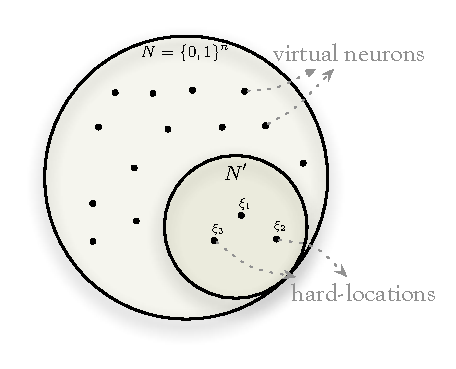
\includegraphics[scale=0.75]{./images02/hardlocations.pdf}

\caption{Hard-locations randomly sampled from binary space.\label{fig-hardlocations}}
\end{figure}


Since a cue $\eta_{x}$ near the target bitstring $\eta$ shares many hard-locations with $\eta$, SDM can retrieve data from imprecise cues. Despite this feature, it is very important to know how imprecise this cue could be while still giving accurate results. What is the maximum distance from our cue to the original data that still retrieves the right answer? An interesting approach is to perform a read operation with a cue $\eta_{x}$, that is $x$ bits away from the target $\eta$.  Then measure the distance from the read output and $\eta$. If this distance is smaller than $x$ we are converging. Convergence is simple to handle, just read again and again, until it converges to the target $\eta$. If this distance is greater than $x$ we are diverging. Finally, if this distance equals $x$ we are in a tip-of-the-tongue process.  A tip-of-the-tongue psychologically happens when you know that you know, but you can't say what exactly it is. In SDM mathematical model, a tip-of-the-tongue process takes infinite time to converge. \citet{Kanerva1988} called this $x$ distance, where the read's output averages $x$, the critical distance. Intuitively, it is the distance from which smaller distances converge and greater distances diverge. In Figure \ref{fig-p1-p2-iterative-read}, the circle has radius equal to the critical distance and every $\eta_{x}$ inside the circle should converge.  The figure also shows a convergence in four readings.

\begin{figure}[!htb]
\centering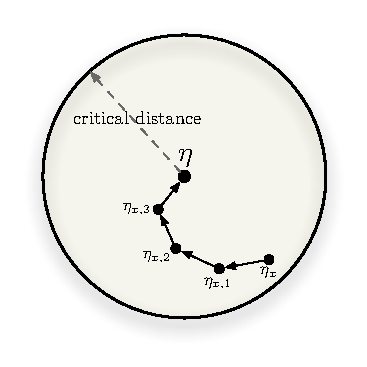
\includegraphics[scale=0.75]{./images02/p1_p2_iter_read.pdf}

\caption{In this example, four iterative readings were\protect \\
required to converge from $\eta_{x}$ to $\eta$.\label{fig-p1-p2-iterative-read}}
\end{figure}


The $\{0,1\}^{n}$ space has $N=2^{n}$ locations from which we instantiate $N'$ samples. Each location in our sample is called a hard-location.  On these hard-locations we do operations of read and write. One of the insights of SDM is exactly the way we read and write: using data as addresses in a distributed fashion. Each datum $\eta$ is written in every activated hard-location inside the access radius centered on the address, that equals datum, $\xi=\eta$. Kanerva suggested using an access radius $r$ having about one one thousandth of $N'$.  As an imprecise cue $\eta_{x}$ shares hard-locations with the target bitstring $\eta,$ it is possible to retrieve $\eta$ correctly. (Actually, probably more than one read is necessary to retrieve exactly $\eta.)$.  Moreover, if some neurons are lost, only a fraction of the datum is lost and it is possible that the memory can still retrieve the right datum.

A random bitstring is generated with equal probability of $0$'s and $1$'s in each bit. One can readily see that the average distance between two random bitstrings has binomial distribution with mean $n/2$ and standard deviation $\sqrt{n/4}$. For a large $n$, most of the space lies close to the mean and has fewer shared hard-locations.  As two bitstrings with distance far from $n/2$ are very improbable, \citet{Kanerva1988} defined that two bitstrings are orthogonal when their distance is $n/2$.

The write operation needs to store, for each dimension bit which happened more ($0$'s or $1$'s). This way, each hard-location has $n$ counters, one for each dimension. The counter is incremented for each bit $1$ and decremented for each bit $0$. Thus, if the counter is positive, there have been more $1$'s than $0$'s, if the counter is negative, there have been more $0$'s than $1$'s, and if the counter is zero, there have been an equal number of $1$'s and $0$'s. Table \ref{tab:write operation} shows an example of a write operation being performed in a 7-dimensional memory.

\begin{table}
\begin{tabular}{c|c|c|c|c|c|c|c|}
\cline{2-8}
$\eta$ & 0 & 1 & 1 & 0 & 1 & 0 & 0\tabularnewline
\cline{2-8}
$\xi_{\textit{before}}$ & 6 & -3 & 12 & -1 & 0 & 2 & 4\tabularnewline
\cline{2-8}
\multicolumn{1}{c}{} & \multicolumn{1}{c}{\textcolor{red}{\small{}$\Downarrow$ -1}} & \multicolumn{1}{c}{\textcolor{red}{\small{}$\Downarrow$ +1}} & \multicolumn{1}{c}{\textcolor{red}{\small{}$\Downarrow$ +1}} & \multicolumn{1}{c}{\textcolor{red}{\small{}$\Downarrow$ -1}} & \multicolumn{1}{c}{\textcolor{red}{\small{}$\Downarrow$ +1}} & \multicolumn{1}{c}{\textcolor{red}{\small{}$\Downarrow$ -1}} & \multicolumn{1}{c}{\textcolor{red}{\small{}$\Downarrow$ -1}}\tabularnewline
\cline{2-8}
$\xi_{\textit{\textit{after}}}$ & \textbf{5} & \textbf{-2} & \textbf{13} & \textbf{-2} & \textbf{1} & \textbf{1} & \textbf{3}\tabularnewline
\cline{2-8}
\end{tabular}

\caption{Write operation example in a 7-dimensional memory of data $\eta$
being written to $\xi$, one of the activated addresses.\label{tab:write operation}}


\end{table}


The read is performed polling each activated hard-location and statistically choosing the most written bit for each dimension. It consists of adding all $n$ counters from the activated hard-locations and, for each bit, choosing bit 1 if the counter is positive, choose bit 0 if the counter if negative, and randomly choose bit 0 or 1 if the counter is zero.


\section{Neurons as pointers}

One interesting view is that neurons in SDM work like pointers. As we write bitstrings in memory, the hard-locations' counters are updated and some bits are flipped. Thus, the activated hard-locations do not necessarily point individually to the bitstring that activated it, but together they point correctly. In other words, the read operation depends on many hard-locations to be successful. This effect is represented in Figure \ref{fig-p1-pointers}: where all hard-locations inside the circle are activated and they, individually, do not point to $\eta$.  But, like vectors, adding them up points to $\eta$. If another datum $\nu$ is written into the memory near $\eta$, the shared hard-locations will have information from both of them and would not point to either.  All hard-locations outside of the circle are also pointing somewhere (possibly other data points). This is not shown, however, in order to keep the picture clean and easily understandable.

\begin{figure}[!htb]
\centering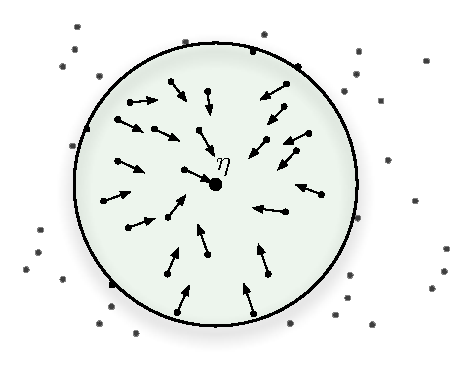
\includegraphics[scale=0.75]{./images02/p1_after_write.pdf}

\caption{Hard-locations pointing, approximately, to the target bitstring.\label{fig-p1-pointers}}
\end{figure}



\section{Concepts}

Although Kanerva does not mention concepts directly in his book \citep{Kanerva1988}, the author's interpretation is that each bitstring may be mapped to a concept. Thus, unrelated concepts are orthogonal and concepts could be linked through a bitstring near both of them. For example, ``beauty'' and ``woman'' have distance $n/2$, but a bitstring that means ``beautiful woman'' could have distance $n/4$ to both of them. As a bitstring with distance $n/4$ is very improbable, it is linking those concepts together. \citet{Linhares2011} approached this concept via ``chunking through averaging''.

Due to the distribution of hard-locations between two random bitstrings, the vast majority of concepts is orthogonal to all others. Consider a non-scientific survey during a cognitive science seminar, where students asked to mention ideas unrelated to the course brought up terms like birthdays, boots, dinosaurs, fever, executive order, x-rays, and so on. Not only are the items unrelated to cognitive science, the topic of the seminar, but they are also unrelated to each other.

For any two memory items, one can readily find a stream of thought relating two such items (``Darwin gave dinosaurs the boot''; ``she ran a fever on her birthday''; ``isn't it time for the Supreme Court to x-ray that executive order?'', ... and so forth). Robert French presents an intriguing example in which one suddenly creates a representation linking the otherwise unrelated concepts of ``coffee cups'' and ``old elephants'' \citep{French1997}.

This mapping from concepts to bitstrings brings us two main questions: (i) Suppose we have a bitstring that is linking two major concepts.  How do we know which concepts are linked together? (ii) From a concept bitstring how can we list all concepts that are somehow linked to it? This second question is called the problem of spreading activation.


\section{Read operation}

In his work, Kanerva proposed and analyzed a read algorithm called here Kanerva's read. His read takes all activated hard-locations counters and sum them. The resulting bitstring has bit $1$ where the result is positive, bit $0$ where the result is negative, and a random bit where the result is zero. In a word, each bit is chosen according to all written bitstrings in all hard-locations, being equal to the bit more appeared. Table \ref{tab:kanerva-read} shows an example of Kanerva's read result bitstring.

Daniel Chada, one member of our research group, proposed another way to read in SDM, in this work called Chada's read. Instead of summing all hard-location counters, each hard-location evaluates its resulting bitstring individually. Then, all resulting bitstrings are summed again, and the same rule as Kanerva applies. Table \ref{tab:chada-read} shows an example of Chada's read result bitstring. The counter's values are normalized to 1, for positive ones, or -1, for negative ones, and the original values are the same as in Table \ref{tab:kanerva-read}.

The main change between Kanerva's read and Chada's read is that, in the former, a hard-location that has more bitstrings written has a greater weight in the decision of each bit. In the latter, all hard-locations have the same weight, because they can contribute to the sum with only one bitstring.

A member of my Master's committee, professor Paulo Murilo, has proposed a generalized reading operation (personal communication), which covers both Kanerva's and Chada's read --- and opens a new venue of potential discoveries. He proposed summing all hard-location counters raised to the power of $z$ while holding the original sign of the counter (positive or negative). Thus, Kanerva's read would be the same as $z=1$, while Chada's would be the same as $z=0$. Hence, we will here explore how SDM would behave with other values of $z$, such as 0.5, 2, and 3.

\begin{table}
\begin{minipage}[t]{0.5\columnwidth}%
\subfloat[Kanerva's read example\label{tab:kanerva-read}]{%
\begin{tabular}{c|c|c|c|c|c|}
\cline{2-6}
$\xi_{1}$ & -2 & 12 & 4 & 0 & -3\tabularnewline
\cline{2-6}
$\xi_{2}$ & -5 & -4 & 2 & 8 & -2\tabularnewline
\cline{2-6}
$\xi_{3}$ & -1 & 0 & -1 & -2 & -1\tabularnewline
\cline{2-6}
$\xi_{4}$ & 3 & 2 & -1 & 3 & 1\tabularnewline
\hline
\multicolumn{1}{|c|}{\textbf{$\sum$}} & \textbf{-5} & \textbf{10} & \textbf{4} & \textbf{3} & \textbf{-5}\tabularnewline
\hline
\multicolumn{1}{c}{} & \multicolumn{1}{c}{\textcolor{red}{\small{}$\Downarrow$}} & \multicolumn{1}{c}{\textcolor{red}{\small{}$\Downarrow$}} & \multicolumn{1}{c}{\textcolor{red}{\small{}$\Downarrow$}} & \multicolumn{1}{c}{\textcolor{red}{\small{}$\Downarrow$}} & \multicolumn{1}{c}{\textcolor{red}{\small{}$\Downarrow$}}\tabularnewline
\cline{2-6}
 & 0 & 1 & 1 & 1 & 0\tabularnewline
\cline{2-6}
\end{tabular}

}%
\end{minipage}%
\begin{minipage}[t]{0.5\columnwidth}%
\subfloat[Chada's read example\label{tab:chada-read}]{%
\begin{tabular}{c|c|c|c|c|c|}
\cline{2-6}
$\xi_{1}$ & -1 & 1 & 1 & \cellcolor{lightgray}1 & -3\tabularnewline
\cline{2-6}
$\xi_{2}$ & -1 & -1 & 1 & 1 & -1\tabularnewline
\cline{2-6}
$\xi_{3}$ & -1 & \cellcolor{lightgray}1 & -1 & -1 & -1\tabularnewline
\cline{2-6}
$\xi_{4}$ & 1 & 1 & -1 & -1 & 1\tabularnewline
\hline
\multicolumn{1}{|c|}{\textbf{$\sum$}} & \textbf{-2} & \textbf{1} & \textbf{0} & \textbf{0} & \textbf{-2}\tabularnewline
\hline
\multicolumn{1}{c}{} & \multicolumn{1}{c}{\textcolor{red}{\small{}$\Downarrow$}} & \multicolumn{1}{c}{\textcolor{red}{\small{}$\Downarrow$}} & \multicolumn{1}{c}{\textcolor{red}{\small{}$\Downarrow$}} & \multicolumn{1}{c}{\textcolor{red}{\small{}$\Downarrow$}} & \multicolumn{1}{c}{\textcolor{red}{\small{}$\Downarrow$}}\tabularnewline
\cline{2-6}
 & 0 & 1 & \cellcolor{lightgray}1 & \cellcolor{lightgray}1 & 0\tabularnewline
\cline{2-6}
\end{tabular}

}%
\end{minipage}\caption{Comparison of Kanerva's read and Chada's read. Each $\xi_{i}$ is
an activated hard-location and the values come from their counters.
Gray cells' value is obtained randomly with probability 50\%.\label{tab:read-operation}}
\end{table}


\section{Critical Distance}

Kanerva describes the critical distance as the threshold of convergence of a sequence of read words. It is ``the distance beyond which divergence is more likely than convergence''\citep{Kanerva1988}. Furthermore, Kanerva explains that ``a very good estimate of the critical distance can be obtained by finding the distance at which the arithmetic mean of the new distance to the target equals the old distance to the target''\citep{Kanerva1988}.  In other words, the critical distance can be equated as the edge to our memory, the limit of human recollection.

In his book, Kanerva analyzed a specific situation with $n=1000$ ($N=2^{1000}$), 10 million hard-locations, an access-radius of 451 (within 1000 hard-locations in each circle) and 10 thousand writes of random bitstrings in the memory. As computer resources were very poor those days, Kanerva couldn't make a more generic analysis.

Starting from the premise of SDM as a faithful model of human short-term memory, a better understanding of the critical distance may shed light on our understanding of the thresholds that bind our own memory.


\begin{figure}[!htb]
\centering

\subfloat[Kanerva's original model]{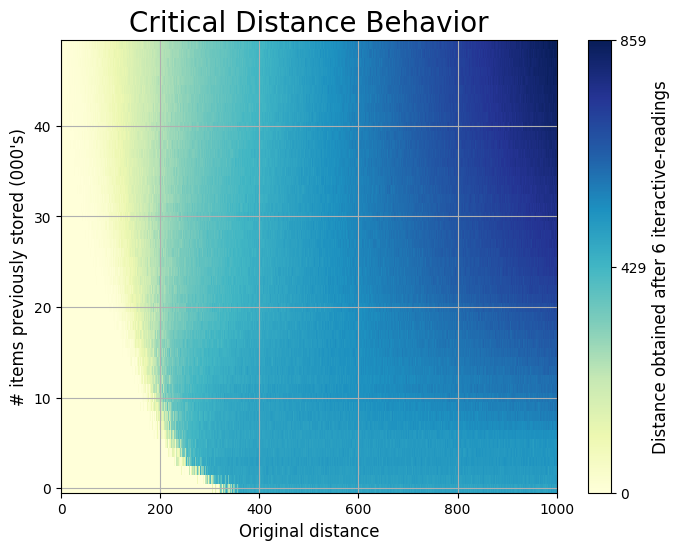
\includegraphics[width=3.1in]{./images02/new-images/kanerva-read.png}}

\subfloat[Chada's read]{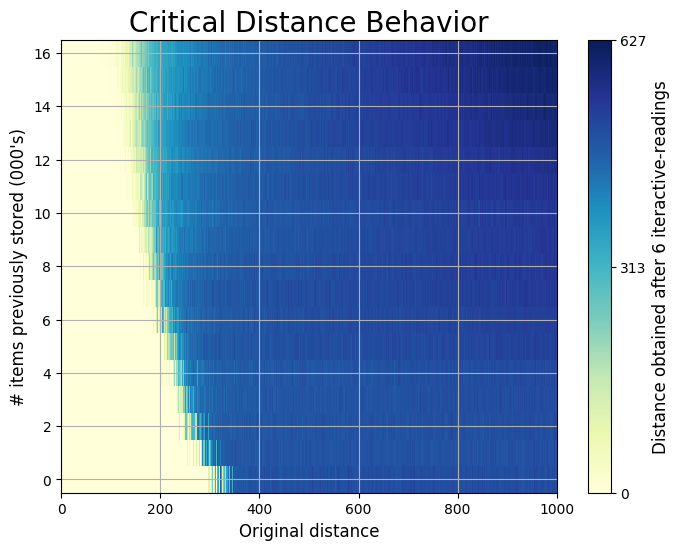
\includegraphics[width=3.1in]{./images02/new-images/chada-read_z_0.png}}
\caption{How far, in hamming distance, is a read item from the original stored item? Kanerva demonstrated that, after a small number of iterative readings (6 here), a critical distance behavior emerges. Items read at close distance converge rapidly; whereas farther items do not converge. Most striking is the point in which the system displays the tip-of-tongue behavior. Described by psychological moments when some features of the item are prominent in one's thoughts, yet the item still cannot be recalled (but an additional cue makes convergence `immediate'). Mathematically, this is the precise distance in which, despite having a relatively high number of cues (correct bits) about the desired item, the time to convergence is infinite.   Heatmap colors display the hamming distance the associative memory is able to cleanly converge to---or not.   In the $x$-axis, the distance from the desired item is displayed. In the $y$-axis, we display the read operation's behavior as the number of items registered in the memory grows.  These graphs are computing intensive, yet they can be easily tested by readers in our provided jupyter notebooks. Note the different scales.}
\label{fig:crit-dist-10k-writes}

\end{figure}

Figure \ref{fig:crit-dist-10k-writes} compares the critical distance behavior under different scenarios.  This replicates our previous results \citet{Brogliato2011} and \citet{brogliato2014sparse} and is a first part of the process of framework validation, to which we throw our attention next.



\chapter{Framework Architecture}

The framework implements the basic operations in a Sparse Distributed Memory which may be used to create more complex operations. It is developed in C language --- which may be loaded in many platforms and programming languages --- with a wrapper in Python. The Python module makes it easy to create and execute operations in a Sparse Distributed Memory.

We split the SDM memory in two parts: the hard-location address space and the hard-location counters. Thus, the addresses (bitstrings) of the hard-locations are stored in one array, while their counters in another. This may be useful to create multiple SDMs using the same address space, which would save computational effort to scan a bitstring in all the SDMs --- since they share the same address space, the activated hard-locations will be same in all of them. As the slowest part of reading and writing operations is scanning the address space, the performance benefits are high.

Each part may be stored either in the RAM memory or in a file. The RAM memory is interesting for quick experiments, automated tests, and others scenarios in which the SDM may be lost. The file is interesting for a long-term SDM --- one may create an SDM file with 10,000 random writes, which will be copied over and over to run multiple experiments. The file may also be sent to another researcher or may be published with the paper to let others run their own checks and verify the results. In summary, the framework fits many different uses and necessities.

There are some other advantages splitting the address space and the counters. When the scanner is run in the CPU, the accessed addresses in the RAM are continuous which improves considerably performance. When the scanner is run in the GPU, only the address space must be uploaded to the GPU, reducing the required memory.

Let a SDM memory with $N$ dimensions and $H$ hard-locations. Then, in a 64-bit computer, the array of hard-location addresses will use $H \cdot 8 \cdot \lceil N/64 \rceil$ bytes of memory, and there will be $H \cdot N$ hard-location counters. For example, in a SDM memory with 1,000 dimensions and 1,000,000 hard-locations, using 16-bit integers for the counters, the array of addresses will use 122MB of memory and the counters will use 1.9 GB of memory.

Basic operations were grouped in four sets: (i) for bitstrings, (ii) for addresses, (iii) for counters, and (iv) for memories (SDMs). Operations include creating new bitstrings, flipping bits, generating bitstring with a specific distance from a given bitstring, scan the address space using different algorithms, write a bitstring to a counter, write in an SDM, read from an SDM, and iteratively read from an SDM until convergence.

\section{Read and write operations}

The reading and writing operations are executed in two steps: first, the address space is swept looking for the activated addresses; then, the operation is performed in the counter. Reading operation assemblies the bitstring according to the counters of the activated addresses, while the writing operation changes the counters.

Counters may have overflow protection depending on compiling options. By default, there is no overflow check in the counters, since each counter is a signed 32-bit integer --- which can store any number integer -2,147,483,648 and 2,147,483,647 --- and they will not overflow with less than $2^31-1$ divided by the number of activated hard-locations. When $N=1,000$, $H=1,000,000$, and $r=451$, the average number of activated hard-locations is 1,000 and it would require at least one million writes to overflow a counter.


\section{Implementation details}

\subsection{The distace between two bitstrings}

The hamming distance between two bitstrings is calculated counting the number of ones in the XOR of the bitstrings, i.e., $d(x, y) = \text{number of ones in} x \oplus y$. In order to count the number of ones of the XOR, the framework uses a pre-calculated table of distances --- by default, it is used a 16-bit table which uses 65MB of RAM, but one may increase to a 32-bit table which uses 4GB of RAM. Finally, to calculate the distance between two bitstrings, it sums the distance of each 16-bit part of the bitstrings, i.e., $d(x[0:N-1], y[0:N-1]) = d(x[0:15], y[0:15]) + d(x[16:31], y[16:31]) + \dots$. As each distance is calculated in O(1), this algorithm runs in O($\lceil bits/16 \rceil$).

The address space is stored in an array of addresses, which, in turn, is stored in arrays of 64-bit integers (Fig. \ref{tab:hl-addresses-detail}). As the addresses and their 64-bit integers are contiguous in RAM or file, there is a performance gain because processors load them in chunks.

\begin{figure}
\centering
\begin{tikzpicture}[
mycell/.style={draw, minimum size=7mm},
matrixA/.style={matrix of nodes,
    nodes={mycell, anchor=center},
    column sep=-\pgflinewidth,
    row sep=-\pgflinewidth,
    },
matrixB/.style={matrix of nodes,
    nodes={mycell, anchor=center},
    column sep=-\pgflinewidth,
    row sep=-\pgflinewidth,
}]

\matrix[matrixA] (A) { addr$_1$ & addr$_2$ & addr$_3$ & $\cdots$ & addr$_H$ \\ };

\matrix[matrixB, below=of A] (B) {
addr$_{k, 1}$ & addr$_{k, 2}$ & addr$_{k, 3}$ & $\cdots$ & addr$_{k, 8 \cdot \lceil N/64 \rceil}$ \\
};

\draw[dashed] (A-1-1.south west)--(B-1-1.north west);
\draw[dashed] (A-1-1.south east)--(B-1-5.north east);
\draw [
	thick,
    decoration={
        brace,
        mirror,
		amplitude=0.2cm,
        raise=0.2cm
    },
    decorate
] (B-1-1.south west) -- (B-1-5.south east)
node [pos=0.5,anchor=north,yshift=-0.5cm] {N bits};

\end{tikzpicture}

\caption{Hard-location addresses are stored in a contiguous array. In a 64-bit computer, each hard-location address is stored in a sub-array of 64-bit integers, with length $8 \cdot \lceil N/64 \rceil$.\label{tab:hl-addresses-detail}}
\end{figure}


\subsection{Scanning for activated hard-locations}

Scanning for the activated hard-locations is a problem similar to well-known problems in computation geometry called ``range reporting in higher dimensions''. In this case, none of the known algorithms is able to solve our problem faster than $O(n)$. The algorithm which seems to best fit in our problem consumes $O(n)$ space and runs in $O(\log^d(n))$ \citep{chazelle1988functional}, which is really slower than $O(n)$ when, for instance, $n=1,000,000$ and $d=1,000$. For a review of the algorithms, see \citet{chan2011orthogonal}.

In 2014, there was published a solution to fast search in hamming space which seems applicable to our problem \citet{norouzi2014fast}.

It is intriguing that none of those algorithms is able to solve our scanning problem. The idea behind those algorithms is roughly to split the search space in half each step, which would take $O(\log(n))$ to go through the whole space. But this approach does not work in our case because of the high number of dimensions (i.e., 1,000) and because the hardlocations' addresses are randomly sampled from the ${0, 1}^d$ space. So, each addresses' bit itself splits the hardlocations in half, but it does not split the search space in half since both halves still must be convered. For instance, let's say we have 1,000 dimensions with 1,000,000 hardlocations, and we are scanning within a circle with radius 451, then after checking the first bit we have two cases: (i) for the half with the same first bit, we must keep scanning with radius 451; and (ii) for the half with a different first bit, we must keep scanning with radius 450. The search space has not been split in half because both halves have been covered (and one of them should have been skipped).

Hence, as our best approach approach seems to be scanning through all hardlocations, we may distribute the scan into many tasks which will be executed independently. The tasks may be executed in different processes, threads, or even computers. They may also run in the CPU or in the GPU. In this case, we may take into account both the time required to distribute the tasks and the time to receive their results.

The framework implements three main scanner algorithms: linear scanner, thread scanner, and OpenCL scanner. The linear scanner runs in a single core, is the slowest one, and was developed only for testing purposes; the thread scanner runs at the CPU in multiple threads sharing memory (and our recommendation is to use the number of threads equals to twice the number of CPU cores); and the OpenCL scanner runs in multiple GPU cores and support multiple devices. The speed of a scan depends on the CPU and GPU devices, thus the best approach to choose which scanner is best for one's setup is to run a benchmark.

The OpenCL must be initialized, which just copies the hardlocations' addresses to the GPU's memory. Then, many scans may be executed with no necessity to upload the addresses again.


\section{Framework Validation}

The framework has been validated comparing its results with the expected results from \citet{Kanerva1988}. Thus, we run simulations which were then compared to the theoretical analysis conducted some decades ago.

SHOW THE RESULTS --- Kanerva's tables/figures vs Simulation.

The objective here is twofold: (i) a single command will install the framework, and (ii) another single command will run (and display) the desired figures obtained the simulation. This will allow potential users to become familiarized with the system and its underlying code with barely any learning curve.

One particular analysis of interest is that of the distance read at a point $\alpha$. Suppose an SDM is trying to read an item written at $\alpha$, but the cues received so far lead to a point of distance $d$ from $\alpha$.  As one reads at $\alpha+d$, a new bitstring $\beta$ is obtained, leading to our question: what is the new distance from $\alpha$ to $\beta$? Is it smaller or larger than $d$? That, of course, depends on the ratio between $d$ and the number of dimensions of the memory.  As we have found out, there are some deviations from Kanerva's original theoretical analysis and the results obtained by simulation.

\subsection{Some initial anomalous results}

As we ran the simulations reflecting some of Kanerva's graphs, one in particular struck our attention: The new distances obtained after a read operation were not perfectly predicted by the theoretical model, and we propose that this is due to interaction effects between different attractors.

\citet{Kanerva1988} originally predicted a \textasciitilde 500-bit distance after a point (Fig. \ref{kanerva-table-7-2}). The original prediction considered that the read distance would decline when inside the critical distance in increase afterwards, converging to a \textasciitilde 500-bit distance.  At this point, each read would lead to a different, orthogonal, \textasciitilde 500-bit distance point.

\begin{figure}[h]
\centering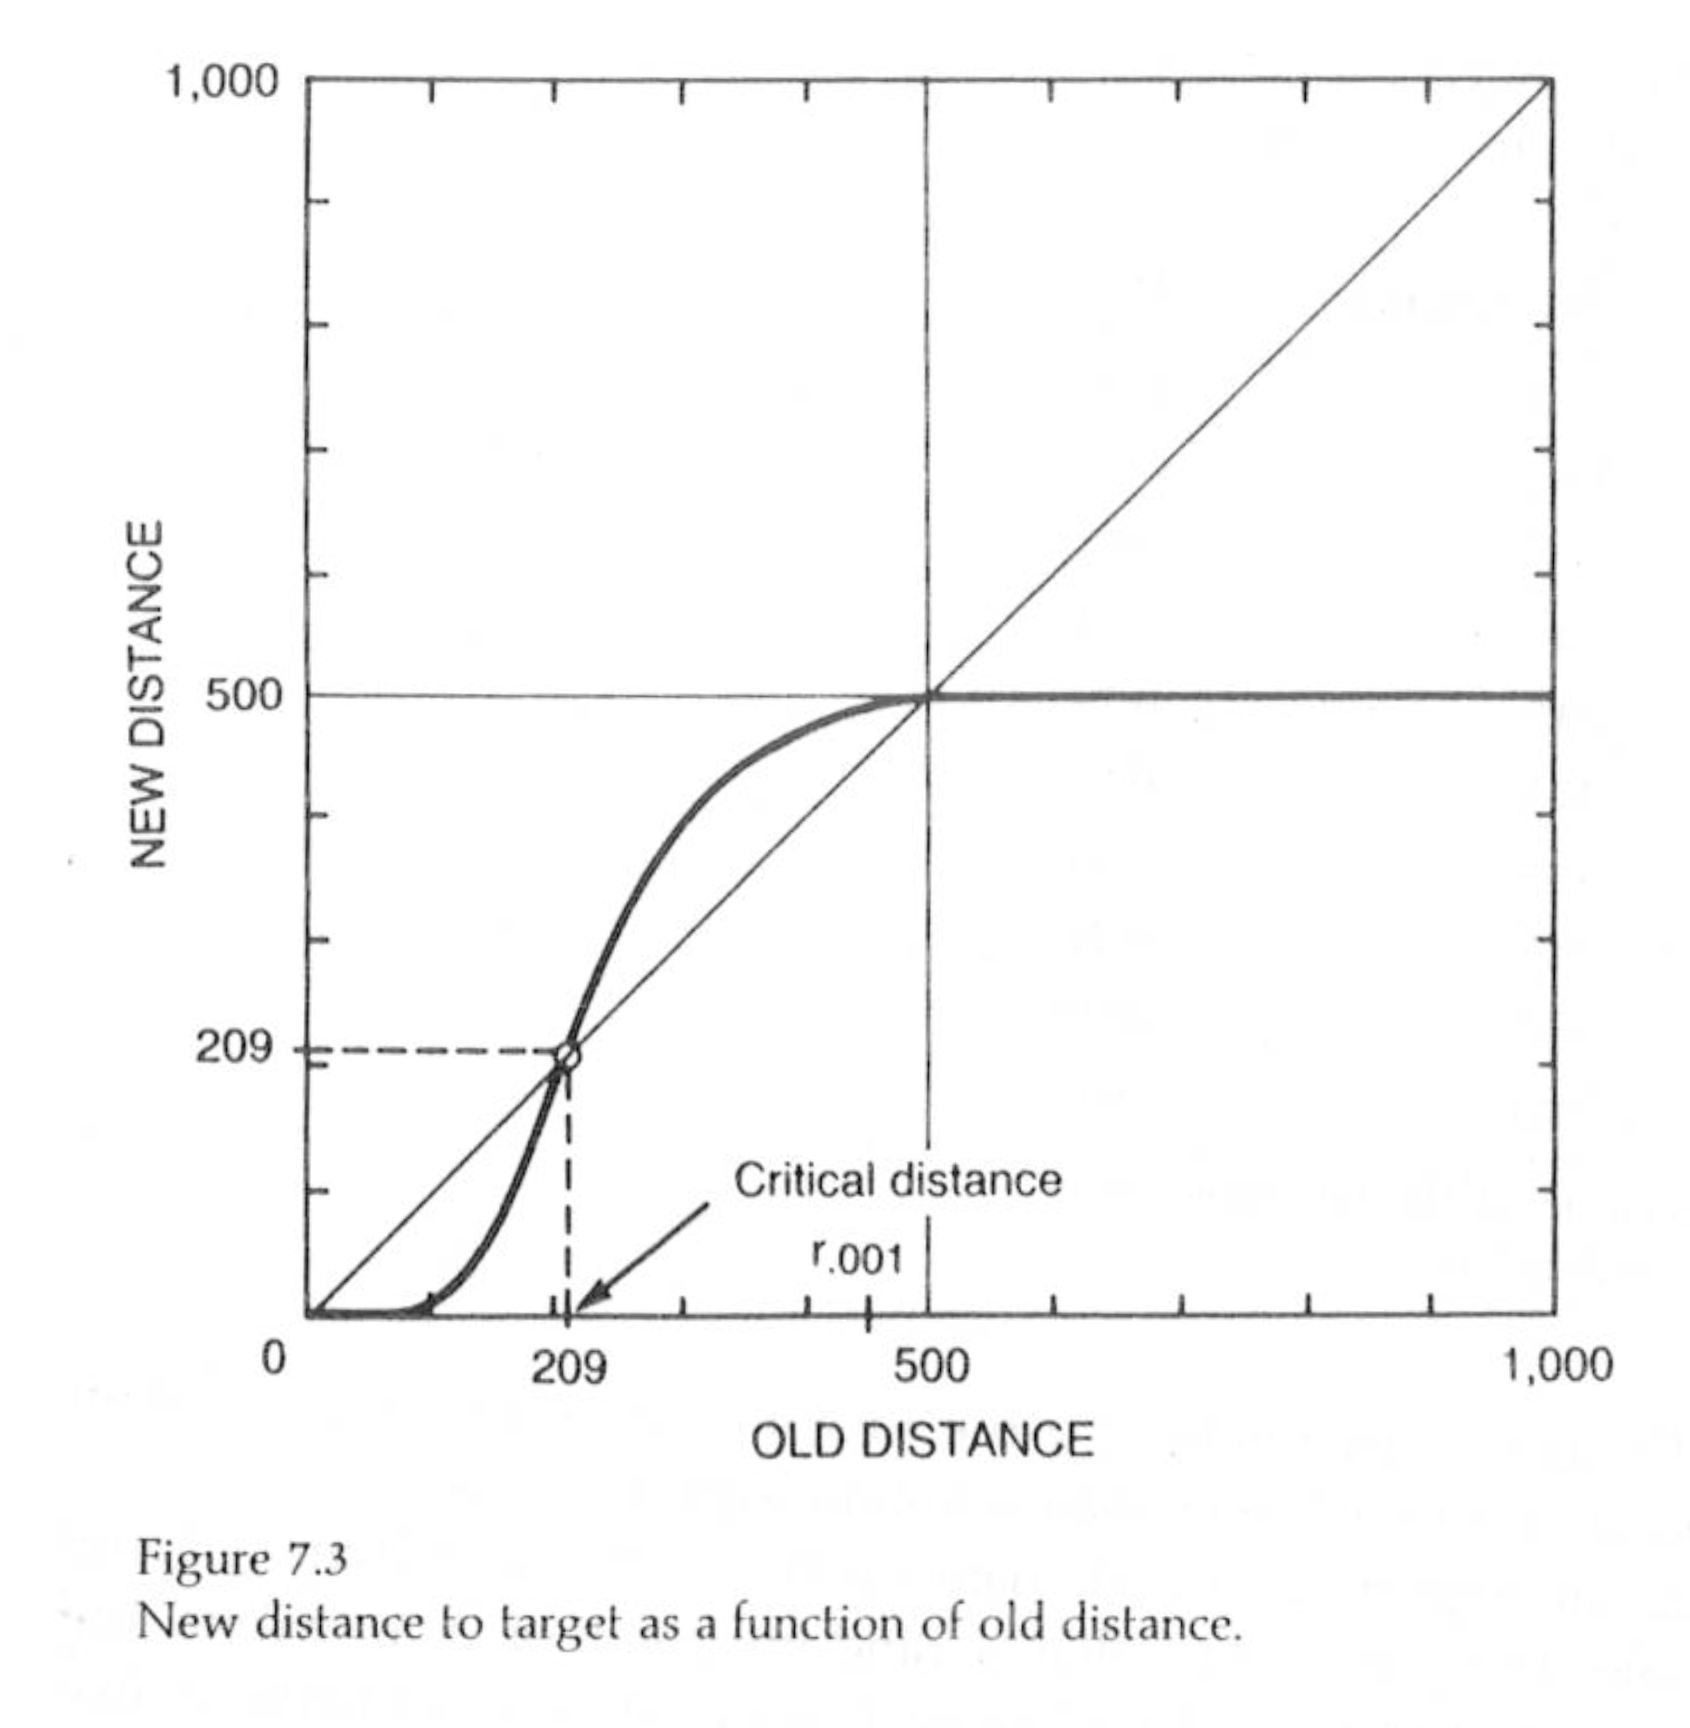
\includegraphics[width=0.5\textwidth]{images02/kanerva-table-7-2-original.png}
\caption{Kanerva's original Figure 7.3 (p. 70) predicting a \textasciitilde 500-bit distance after a point.
\label{kanerva-table-7-2}}
\end{figure}

Our preliminary results show that the theoretical prediction is not accurate.  There are interaction effects from one or more of the attractors created by the 10,000 writes, and these attractors seem to raise the distance beyond \textasciitilde 500 bits (Fig. \ref{sdm-10000w-table-7-2}). Our results were obtained using a 1,000 bit, 1,000,000 hard-location SDM with exactly 10,000 random bitstrings written into it, the same used by Kanerva.

\begin{figure}[h]
\centering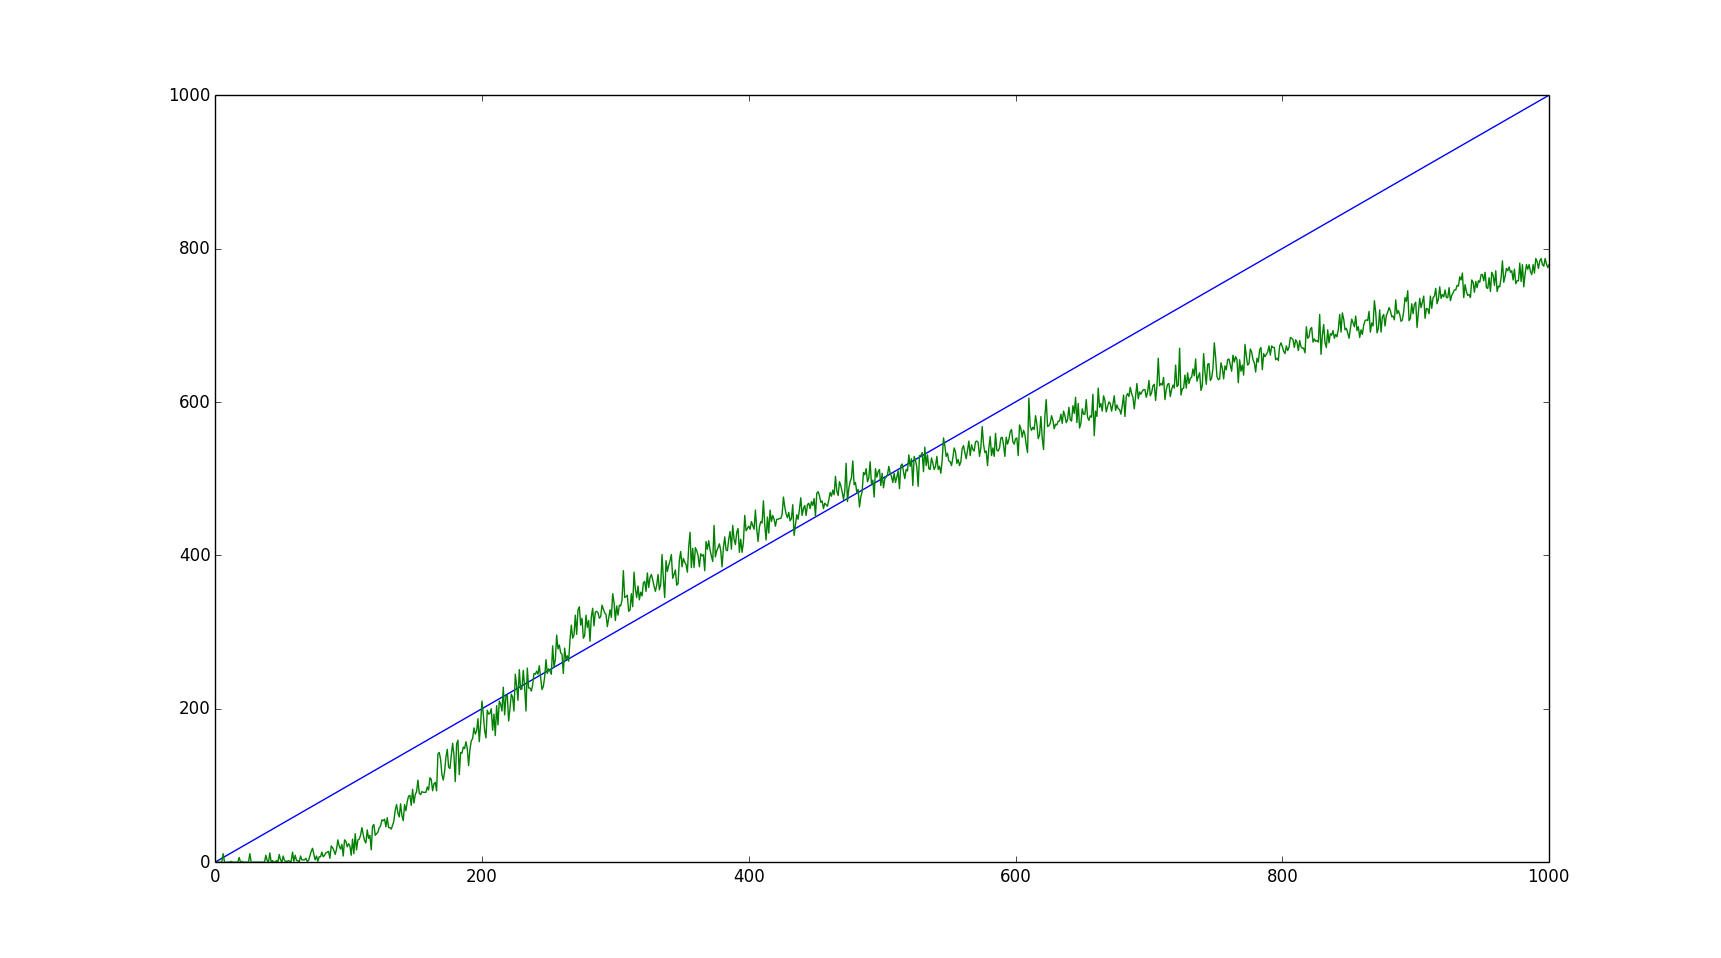
\includegraphics[width=0.5\textwidth]{images02/sdm-10000w-table-7-2.png}
\caption{Results generated by the framework diverging from Kanerva's original Table 7.2. Here we had a 1,000 bit, 1,000,000 hard-location SDM with exactly 10,000 random bitstrings written into it, which was also Kanerva's configuration.
\label{sdm-10000w-table-7-2}}
\end{figure}

But, when we reduced the number of random bitstrings written in the SDM from 10,000 to only 100, the results reflected very well the Kanerva's theoretical expectation (Fig. \ref{sdm-100w-table-7-2}). This result strengthen our theory that the disparities in the computational results are due to the interaction effect of different attractors.

\begin{figure}[h]
\centering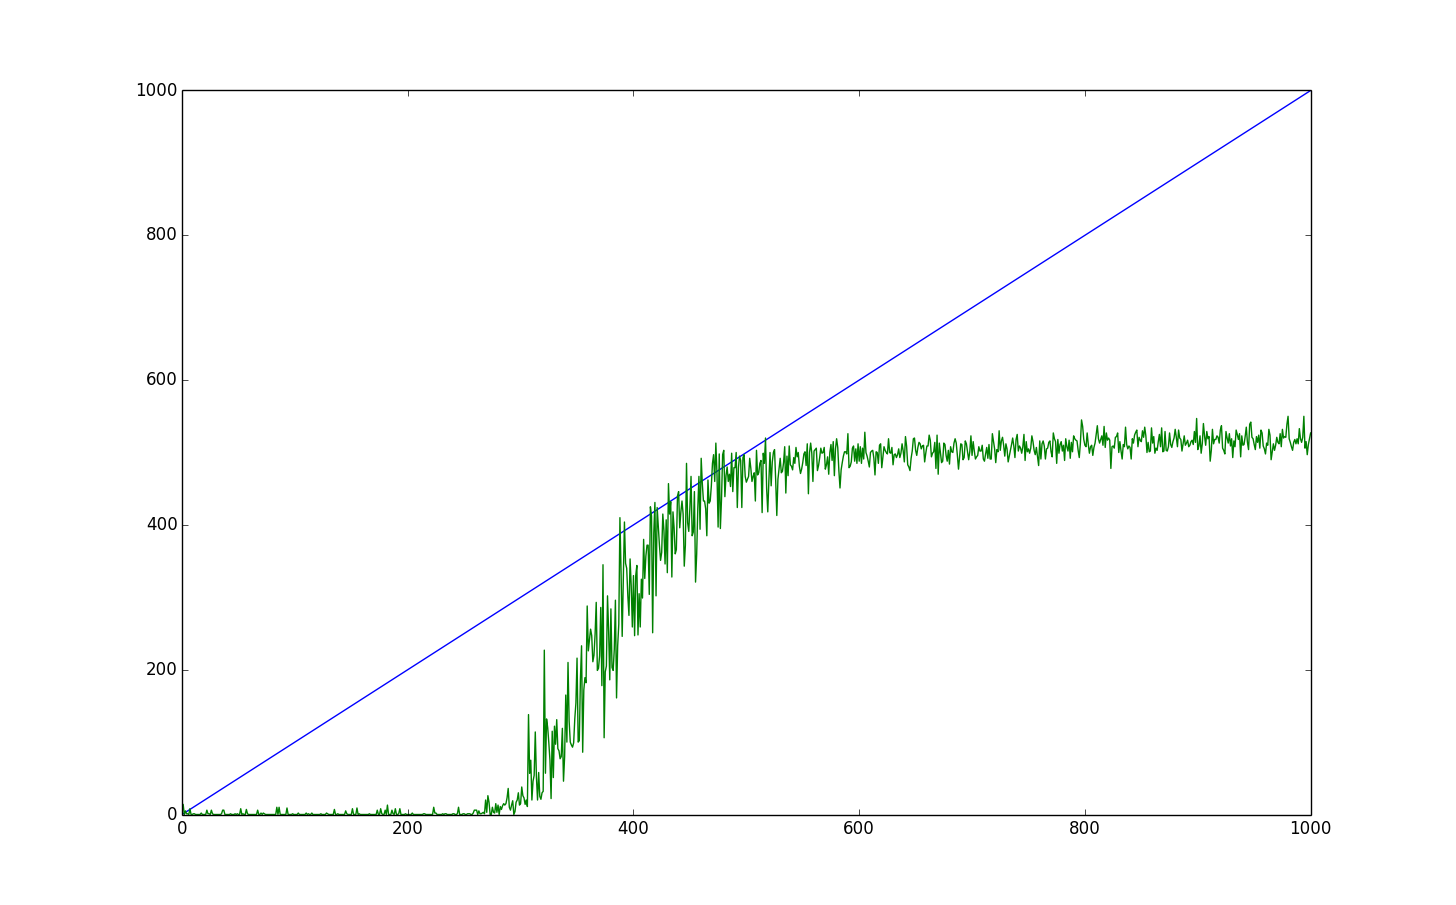
\includegraphics[width=0.5\textwidth]{images02/sdm-100w-table-7-2.png}
\caption{Results generated by the framework similar from Kanerva's original Table 7.2. It was a 1,000 bit, 1,000,000 hard-location SDM with exactly 100 random bitstrings written into it.
\label{sdm-100w-table-7-2}}
\end{figure}

To obtain the results from Fig. \ref{sdm-10000w-table-7-2} and \ref{sdm-100w-table-7-2}, we had to write 10,000 random bitstrings to an SDM, and then randomly choose one of those bitstrings to be our origin. Finally, we randomly flipped some bits from the origin bitstring and executed a reading operation in the SDM. Thereby, in order to show the interaction effects more clearly, we wrote a handmade bitstring to the SDM which had all bits inverted in relation to the origin bitstring --- their hamming distance was equal to 1,000. Our handmade bitstring was acting as an opposite attractor, and one can see the accelerating effects towards convergence to both attractors: the origin and the handmade bitstrings (Fig. \ref{sdm-10000w-notX-table-7-2}). Here we had the exact same configuration of Figure \ref{sdm-10000w-table-7-2}, with the addition of the single opposite attractor.

\begin{figure}[h]
\centering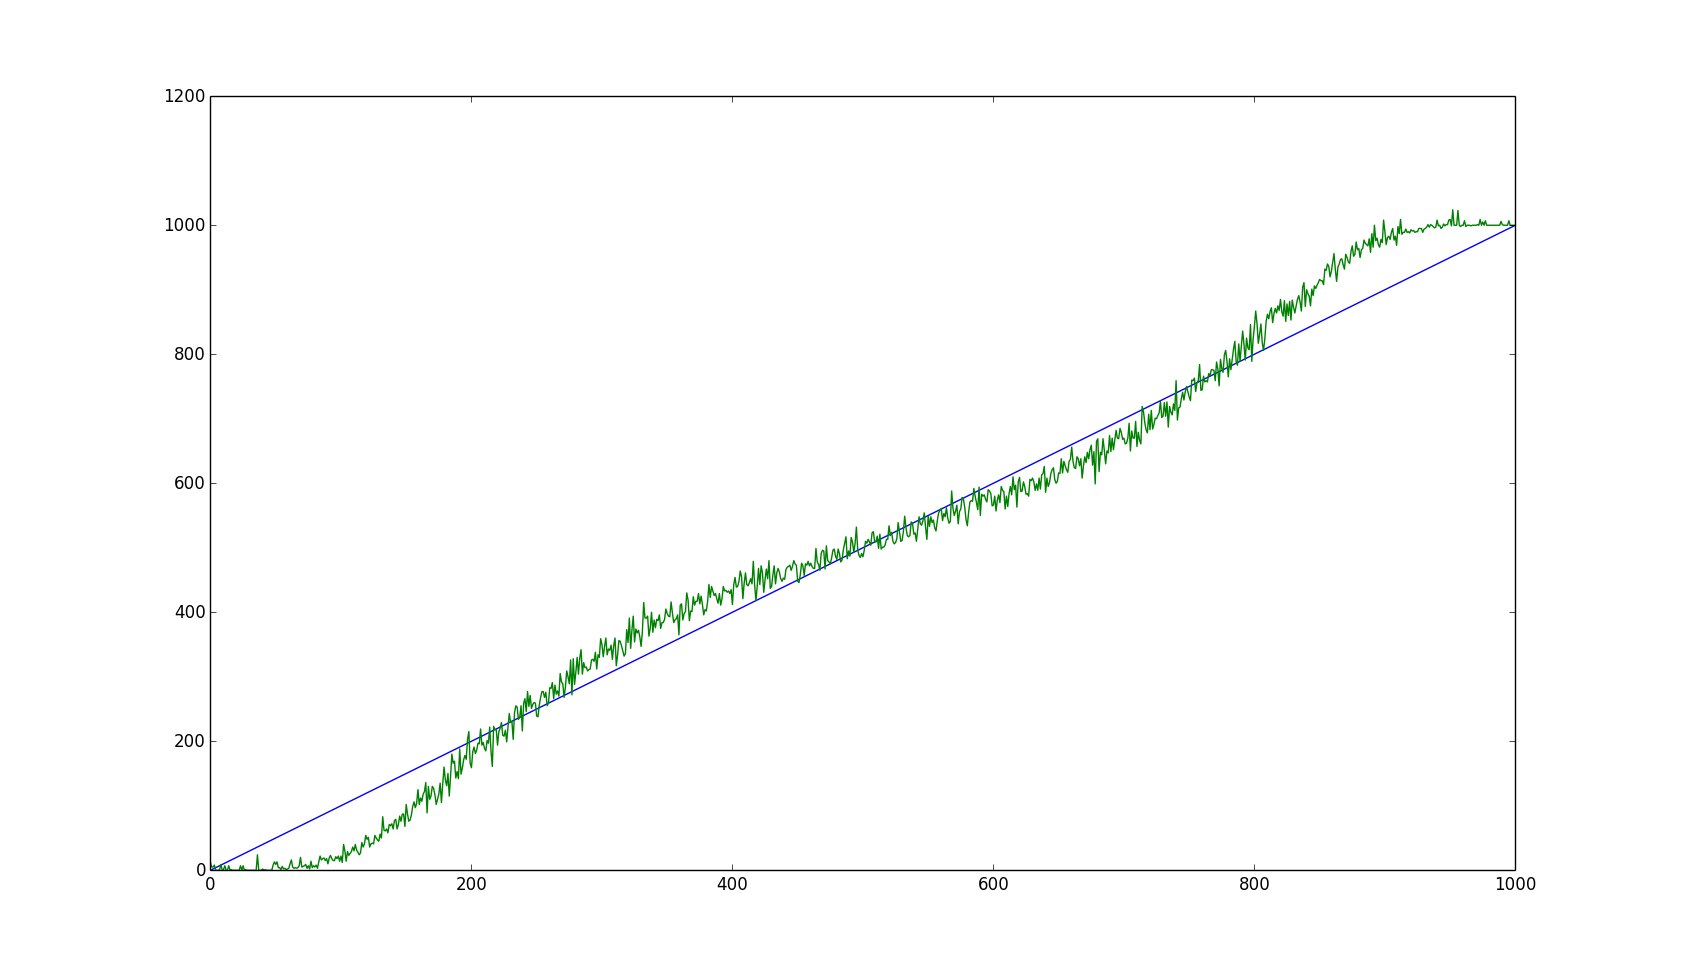
\includegraphics[width=0.5\textwidth]{images02/sdm-10000w-notX-table-7-2.png}
\caption{This graph shows the interaction effects more clearly.  As we include an opposite bitstring, one can see the accelerating effects towards convergence to both attractors: the origin and the opposite. Here we have the exact same configuration of Figure \ref{sdm-10000w-table-7-2}, with the addition of the single opposite attractor.
\label{sdm-10000w-notX-table-7-2}}
\end{figure}

Obviously, these small deviations from Kanerva's original theoretical predictions deserve a qualification.  Kanerva was working in the 1980s and the 1990s, and had no access to the immense computational power that we do today. It is no surprise that some small interaction effects should exist as machines allow us to explore the ideas of his monumental work.

\begin{figure}[h!]
  \centering
  \subfloat[$z \in \{.1, .2, .3, .4, .5, 1\}$]{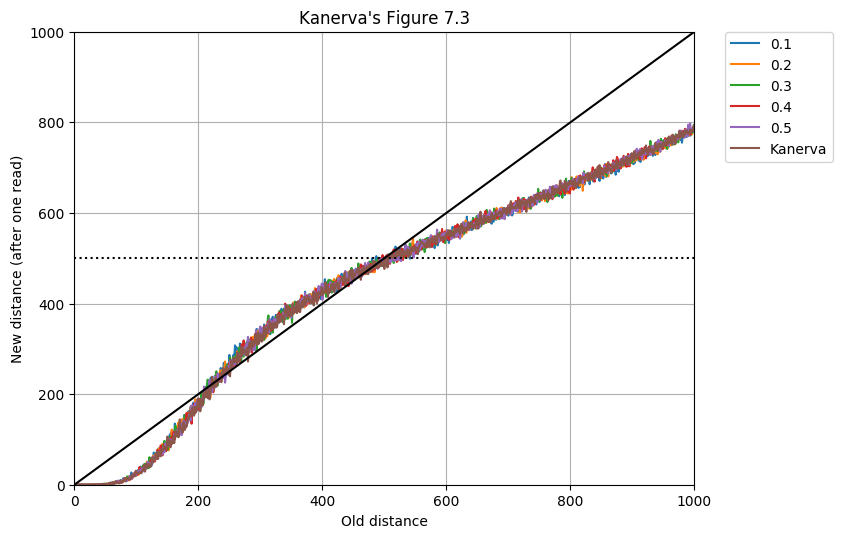
\includegraphics[width=2.9in]{./images02/new-images/iter_z_01-05.png}}
  \subfloat[$z \in \{1.5, 3, 4.5, 6\}$]{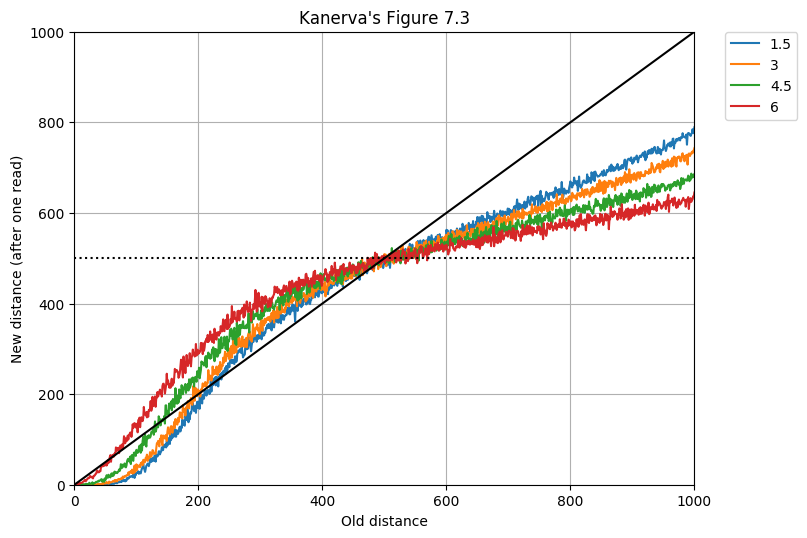
\includegraphics[width=2.9in]{./images02/new-images/z_15_3_45_6.png}}

  \subfloat[$z \in \{0, 1\}$]{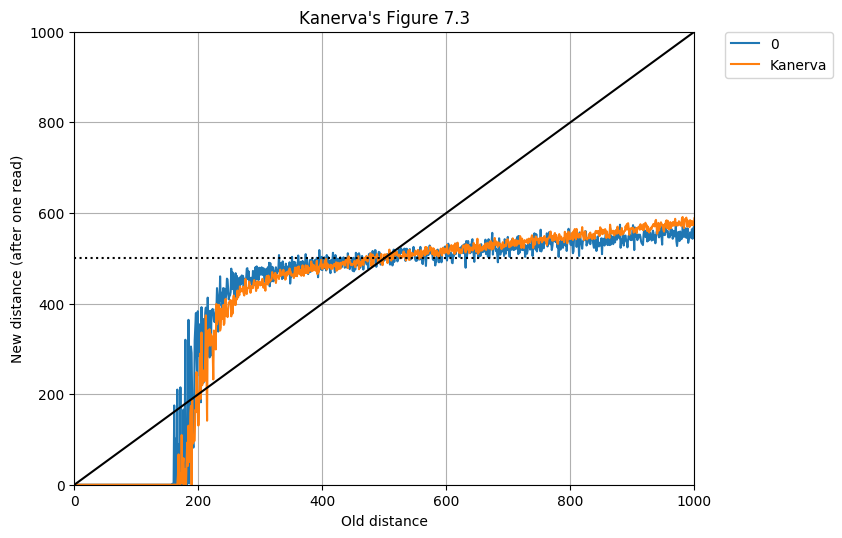
\includegraphics[width=2.9in]{./images02/new-images/z_0_1.png}}
  \subfloat[$z \in \{0, 0.5, 1, 1.5, 3, 4.5, 6\}$]{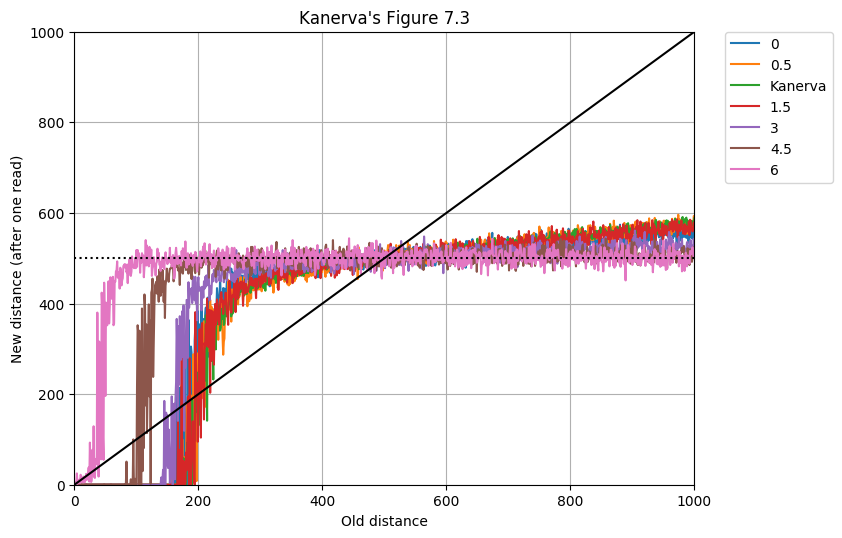
\includegraphics[width=2.9in]{./images02/new-images/iter_z_all_2.png}}

  \caption{(a) and (b) show the behavior of a single read; (c) and (d) present the effects of 6 iterative reads. As stated previously, we can see a deterioration of convergence, with lower critical distance as $z>1$.  Another observation can be made here, concerning the discrepancy of Kanerva's Fig 7.3 and our data.  It seems that Kanerva did not consider that a single read would only `clean' a small number of dimensions \emph{after the critical distance}. What we observe clearly is that with a single read, as the distance grows, the system only `cleans' towards the orthoghonal distance 500 after a number of iterative readings.}
  \label{fig:murillo-generalization-experiments}
\end{figure}

Physicist Paulo Murilo observed that the models of Kanerva-read ($z=1$) and Chada-read ($z=0$) were simple variations of the exponent $z$, which suggests experimenting with different values. The results, however, have not yielded performance improvements.  Though for $z \leq 1$ results are comparable to $z=1$, for $z>1$, the system shows a clear deterioration, with a smaller distance to convergence and higher divergence at large-distance reads. This is shown in Figure \ref{fig:murillo-generalization-experiments}. 



\section{Applications}

\subsection{Noise filter}

We developed a noise filter using a SDM.


\subsection{Classification filter}


\section{Performance Results}

Our intention is to provide comparative performance metrics under different computation engines (CPU, GPU, etc) and different operating systems (Linux, MacOs, Windows, etc). Performance can be measured as the average number of scans of all hard locations per second, reads per second, writes per second, etc.

Our first device is a personal MacBook Pro Retina 13-inch Late 2013 with a 2.6GHz Intel core i5 processor, 6GB DDR3 RAM, and Intel Iris GPU.  We also intend to test on machines such as the iMac with dedicated GPU, MacPro with dedicated GPU, and personal computers under Linux with dedicated GPUs.

Beyond that, we are running as state-of-the-art devices: (i) an Amazon EC2 p3.xlarge with Intel Xeon E5-2686v4 processor, 61GB DDR3 RAM, and NVIDIA K80 GPU, and (ii) an Amazon EC2 p3.8xlarge with Intel Xeon E5-2686v4 processor, 488GB DDR3 RAM, and 8x NVIDIA K80 GPU.


\chapter{Conclusion}

Sparse Distributed Memory is a viable model of human memory, yet it does require researchers to (re-)implement a number of parallel algorithms in different architectures.

We propose to provide a new, open-source, cross-platform, highly parallel framework in which researchers may be able to create hypothesis and test them computationally through minimal effort. Though the framework is not well-documented for public release at this time, it has already served as the backbone of Chada's Ph.D. thesis. The single-line command ``pip install sdm'' will install the framework on posix-like systems, and single-line commands will let users test the framework, generate some of the figures from Kanerva's theoretical predictions in their own machines, and --- if interested enough ---, test their own theories and improve the framework in an open-source fashion. It is our belief that such work is a necessary component towards accelerating research in this promising field.

% TODO Include in the to do list simulations based on the suggestion of Murilinho.

\chapter{Appendix}
\section{Generating Kanerva's table 7.3}

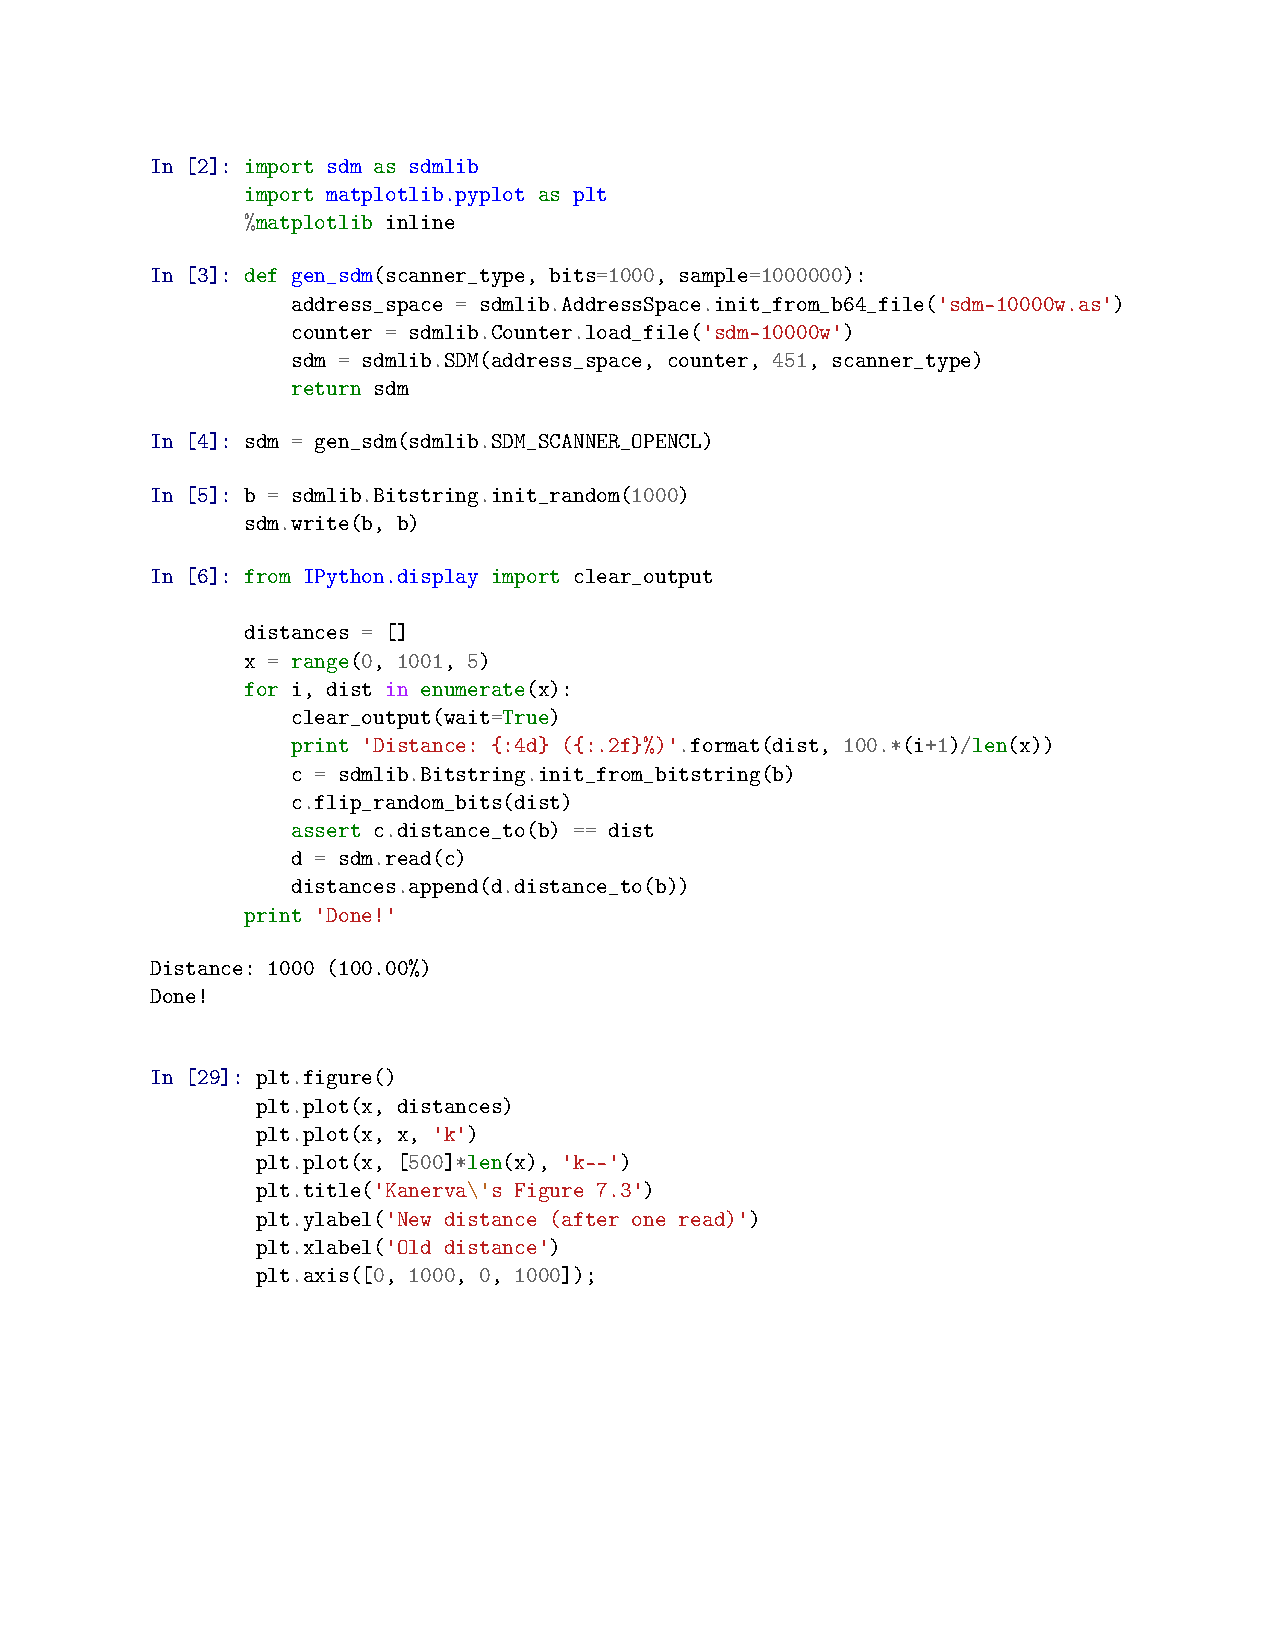
\includepdf[
  pages=-,
  pagecommand={\pagestyle{headings}},
  %addtotoc={1,section,1,Quilling Shapes,sec:shapes}
]{./Chapter02-SDM/Kanerva-Table-7.3/Kanerva-Table-7_3.pdf}
